\section{Introduction}\label{sec-intro}

% Traditional network control approaches relied on simplistic, sometimes
% manual changes to the control planes of distributed network devices to
% achieve various objectives. As a result, they were brittle and slow to
% react  to changes in the underlying network or its traffic patterns.
Software defined networking (SDN) advocates separating control and
data planes in network devices, and provides a logically centralized
platform to program data plane state~\cite{openflow,rethinking}.
This has opened the door to rich network control applications that can
adapt to changes in the underlying network or its traffic patterns
more flexibly and at smaller time scales than legacy control
planes~\cite{swan,b4,ananta,simple,elastictree,softcell}. % For example,
% recent work has shown that WAN networks can be reconfigured in 10s of
% seconds using SDN, whereas legacy protocols may take
% hours~\cite{swan,b4}. \aditya{check this}
Therefore, it is not surprising that SDN is being rapidly deployed or under developed in
many domains, including data center (DC)~\cite{zupdate,microte,elastictree},
cloud~\cite{ananta}, inter-DC WAN~\cite{b4,swan} and,
cellular~\cite{softcell} networks.

%  and even high frequency
% trading~\cite{arista,hp}. 

However, a number of important management applications in these
domains, such as fast fail-over, reactive routing of latency-sensitive
flows, and fine-grained DC traffic engineering~\cite{microte}, are
stretching SDN's capabilities. These applications require the ability
to reprogram data plane state at very fine time-scales to optimally
meet their objectives. For instance,
fine-grained DC traffic engineering approaches require routes to be
set up within a few hundred milliseconds to leverage short-term traffic
predictability~\cite{microte}. Setting up routes in
cellular networks (when a device becomes active, or a during handoff)
must complete within $\sim$30-40ms to ensure users can interact with
Web services in a timely fashion. It is important that SDN support
such applications, otherwise operators will be forced to adopt
expensive custom solutions alongside SDN (e.g., bandwidth reservation,
custom hardware/protocols etc.), which can undermine SDN's ``CapEx''
and ``OpEx'' benefits.

For such applications, timely interaction between the logically
central SDN control plane and network switches is crucial. Timeliness
is determined by: (i) the speed of control programs, and latency
to/from the logically central controller, and (ii) the responsiveness
of network switches in interacting with the controller, specifically,
in generating the necessary input messages for control programs, and then
modifying forwarding state as dictated by them. Robust
control software design and advances in distributed
controllers~\cite{onix} have helped overcome the first issue. However,
with most of the focus today being on the flexibility benefits of SDN
relative to legacy technology, the latter issue has not gained much
attention from vendors and researches alike.

% and is posing problems for some classes of applications today.

% the latter issue has received scant attention. with demanding placing
% stringent demands on controlling data plane state at fine time-scales,
% the latter issue is starting to gain importance. Examples of such
% applications include .

% . Such applications variety of settings, e.g., data center
% (DC)~\cite{microte,hedera,xxx}, cloud~\cite{nicira,ananta},
% enterprise~\cite{ethane,pane:sigcomm13} inter-DC WAN~\cite{swan,B4},
% and cellular~\cite{softcell}. \li{The
%   above does not link to the next
%   paragraph very well. Maybe say something that,} \aditya{fixed.}

% Some important dynamic control applications, such as, require fast interaction between
% controllers and switches. 

% As a result, a number of issues remain poorly understood:Wwhat is the
% magnitude of the latencies underlying switch actions in?  What
% factors determine these latencies? what are the underlying
% causes of the latencies? Are the causes are fundamental to
% switch design? 

Alarmingly, preliminary studies~\cite{ucsdpaper,oflops}
and anecdotal evidence suggest that latencies underlying switch
actions in (ii) could be significant. However, it is not clear what
factors impact these latencies, what the underlying causes are, and
whether the causes are fundamental to switch designs. As a
result, whether it is possible to overcome these latencies at all is
not known. Thus, SDN's ability to provide sufficiently
responsive control to support the aforementioned applications remains
in question.

% Thus, important applications smay be seriously
% impacted.
% % of network This brings SDN-based network control in questionis a significant challenge for control
% % applications, and so it may be tempting to conclude that the
% % responsiveness one can expect from SDN control applications may be
% % limited in practice.

% However, by virtue of centralized view and global control, SDN also
% provides opportunities for mitigating or even overcoming these
% latencies. As a simple example, the controller can constantly probe
% network switches to enable management applications to use the most
% responsive switches. However, the need for and effectiveness of such
%  techniques, as well as the most suitable way to design them, depend
%  on a thorough understanding of
% \li{the above should have a better version} \aditya{yet to
%   fix. previous two paras need fixing}

 To this end, we make two contributions. In this first part,
 we present a thorough systematic exploration of these latencies in production
 SDN switches from 2 different vendors---Broadcom and Intel---using a
 variety of workloads. We investigate the
 relationship between switch design and observed latencies using both
 greybox probes and feedback from vendors.
 Key highlights from our measurements are as follows: (1) We find that
 {\em inbound latency}, i.e., the latency involved in the switch
 generating events (e.g., when a flow is seen for the first time) can
 be high (8 ms per rule on average on Intel). We find the delay is particularly high
 whenever the switch CPU is simultaneously processing forwarding rules
 received from the controller. (2) We find that {\em outbound latency}, i.e., the
 latency involved in the switch installing/modifying/deleting
 forwarding rules provided by control applications, is high as well
 (3ms and 30ms per rule for insertion and modification, respectively,
 in Broadcom). The latency crucially depends on the priority patterns both in rules being inserted as well those already in a switch's table. We find
 that there are significant differences in latency trends across the two
 switches, pointing to different internal optimizations.

%  However, the magnitudes depend both on switch designs and rule priorities.
% : for example,
%  inserting a burst of 50 equal priority rules into a switch can take
%  up to 100ms, and
%  the latency grows linearly with burst size.
%  (3) We find that when priorities are involved, outbound
%  latencies can be quite
%  high, running into seconds depending on the pattern of rule
%  priorities; e.g., the above latency shoots up to XXXms, a factor of XXX. %  For example, installing 50 high priority rules into a
 % table containing 100 low priority rules can take up to XXXms. \aditya{time outs, poll stats, deletions, modifications}

 We find that poor switch software design contributes significantly to
 the observed high latencies. However, pathological interactions between
 some rule priority input sequences and switch hardware table  heuristics for
 rule layout play a significant  role in inflating latency as well.
 Crucially, the latter issue is  fundamental and may be hard to overcome.
%  difficult to avoid over time.

% While we expect switch software to improve over time, our interactions
% with the operators indicate thatthere will
% likely be implementation issues that, coupled with fundamental traits
% of hardware, will always lead to non-trivial latencies. 

%\aditya{need something here}
 Informed by our measurements, we
 design a framework called Mazu that {\em leverages} the centralized view
 and global control in SDN to overcome or mitigate the impact of
 latencies, including both latencies from implementation-related causes
 and those from fundamental ones. % Mazu uses a clever combination of
%  {\em  functionality decoupling}, {\em workload
%   engineering}, and {\em probing} to simultaneously target both the
% fundamental as well as implementation-related contributors
% to latencies.
% \li{readers will not be able to understand what the three techniques mean. Need
%   to explain them in place.}
 The first technique in Mazu is to avoid the switch CPU processing
 events due to data plane packet arrivals by redirecting packets to a
 fast proxy that is tasked with generating the necessary messages for the
 controller. By leveraging a fast commodity processor and decoupling
 inbound and outbound actions, this eliminates inbound latency.
 
Because
 outbound latency is intrinsically linked to switch
 software and hardware,
% due to its intrinsic relation to switch software and
% hardware
 we develop techniques that can be used (in
 isolation or together) for systematically {\em mitigating} it. Our
 first technique, {\em flow engineering}, leverages our empirical latency models to  compute paths such
 that the latency of installing forwarding state at any switch is minimized. Our second
 technique, {\em
   rule offloading}, computes strategies for opportunistically
 offloading portions of
 forwarding state to be installed at a switch to other switches
 downstream from it. By virtue of reducing installation latency per switch and enabling parallel execution of updates,
 these two techniques ensure rule update tasks to
 finish much faster. Finally, we provide rules for installation at a switch in an
 order that is optimal for the vendor in question. 

 We evaluate these techniques for fast fail-over and responsive
 traffic engineering applications under various settings. Depending on
 the topology and the nature of rules in switches, we find that
in/outbound latencies can render SDN incapable of supporting such
applications. In contrast, 
our techniques can
 improve the time taken to update network state in these scenarios by factors
 of 1.6-5X, which we argue makes SDN-based control suitably responsive for these
 settings.

% \aditya{what about priority insertion}

% \aditya{this will go: Our final technique, multipath probing,
%  sets up multiple paths in parallel so that data plane packets can be
%  switched in hardware as soon as one path completes its setup.  This
%  mechanism deals with unexpected delays imposed by switch CPU (e.g.,
%  due to CPU  processing
%  of other tasks such as polling statistics) and hardware (e.g., due to
%  TCAM reorganization).}

%  \aditya{some sentences
%   in this para will have to
%   be  rewritten}

% \aditya{rest is to do}

% % Finally, we control the actual
% % installation of flows at edge and core switches by reordering them
% % according to priority.\aditya{check this XXX}\marina{is there a
% %   batching of the rules as well before determining order}

% \iffalse

% In some situations, the t\_out latencies may be impacted by other
% factors that cannot be controlled; e.g., when an application is
% attempting to reactively install routes while another is reading
% statistics from existing switches. While the above approaches help
% reduce latency somewhat in such situations, there is still enough
% variation in the latencies that flows can face.
%  meeasurements do not unearth. To account for these, we introduce an
%  opportunistic multipath probing scheme that explores up to
%  $k$ candidate paths between a source destination pair \marina{these paths are based on existing rule sets in the switches?}, taking
%  into account potential interference across pairs. The schemes selects
%  one path per pair such that the t\_out delay experienced by all pairs
%  is minimized. \aditya{need to finish. need a lot more detail.}


 
% However, it is not clear what factors cause such high latencies and
% whether the causes are fundamental to design. Equally importantly, 

% arise
% However, it is not
% known why the latencies arise, whether the underlying causes are
% fundamental However, it is not known how the latencies manifest under
% various workload conditions and across a variety of platforms, what
% underlying issues contribute to them, and whether these issues are
% fundamental to switch designs today.


% % While SDN has certainly made the control planes richer and more
% % robust, it introduces a new complexity: the control plane can impact
% % the performance of the data plane on fine time-scales. 

% %  twist to how the control plane affects
% % data plane performance. In traditional networks, the control plane's
% % poor adaptation lead to the data plane doing useless work (e.g.,
% % packets looping during convergence) or being not fully utilized. In
% % SDNs, however, the data plane performance is impacted on fine
% % time-scales because of 

% % challenges

% But exactly how responsive is SDN-based network control? Consider the
% example where an OpenFlow-based SDN application is trying to
% reactively establish routes for flows within the data center, e.g., in
% response to a failure. The actions involved are shown in Figure XXX
% for a simplified network with a single switch.\marina{Is this Fig same
%   as Fig 1, also include numbering on fig to show sequence of flow set
%   up process} Notice that the actual forwarding for the flow in
% question does not begin until t\_in + t\_out seconds. If the latency
% introduced by the network is ignored, then t\_in and t\_out are driven
% purely by the ability of SDN switches to quickly execute SDN-related
% actions.

% Most existing SDN approaches assume that these latencies are
% negligible. This would be possible in a world where SDN switch
% software and chip designs are highly optimized to support SDN-based
% actions. In practice, however, poor software designs, unoptimized
% hardware paths, and fundamental traits of memory hardware conspire to
% cause the latencies to be significantly higher!

% In~\figref{openflow_switch_delay}, we show a deeper view into an SDN
% switch, various actions the switch takes, and how they contribute to
% t\_in and t\_out. As the figure indicates, the latencies t\_in and
% t\_out depend on key aspects of the switch's design including how the
% switch software processes different messages, the software's
% interaction with the switch hardware table (typically a TCAM), and the
% corresponding actions taken by the hardware table's SDK. These aspects
% may be exercised to different extents based on switch workload, such
% as the nature of the rule being installed (simple 5-tuple based vs
% complex rule based on the entire OpenFlow 10-tuple), the rule's
% priority relative to those already installed, size of the currently
% installed rule base, rate at which the controller is simultaneously
% pushing other rules to the switch and the nature of those rules, etc.

% To date, not much attention has been paid to estimating these
% latencies in the wild under various workloads, and analyzing the
% impact of switch designs on the latencies. \marina{Place UCSD paper into context} Understanding these is
% crucial to how SDN is used: it can inform operators on whether certain
% SDN approaches (such as the reactive failure avoidance approach above)
% can offer close to the promised benefits given current switches on the
% market. It can also inform them on how best to avoid or mitigate the
% impact of the latencies on their applications. To switch and chip
% vendors, it can highlight what aspects of their software and SDK
% designs can be improved to support faster actions.
% % how to alter SDN switch designs where possible to address the latencies, and how to develop SDN applications that modulate switch workloads to avoid being impacted by the latencies.

% \begin{figure}[!tb]
% \centering
% %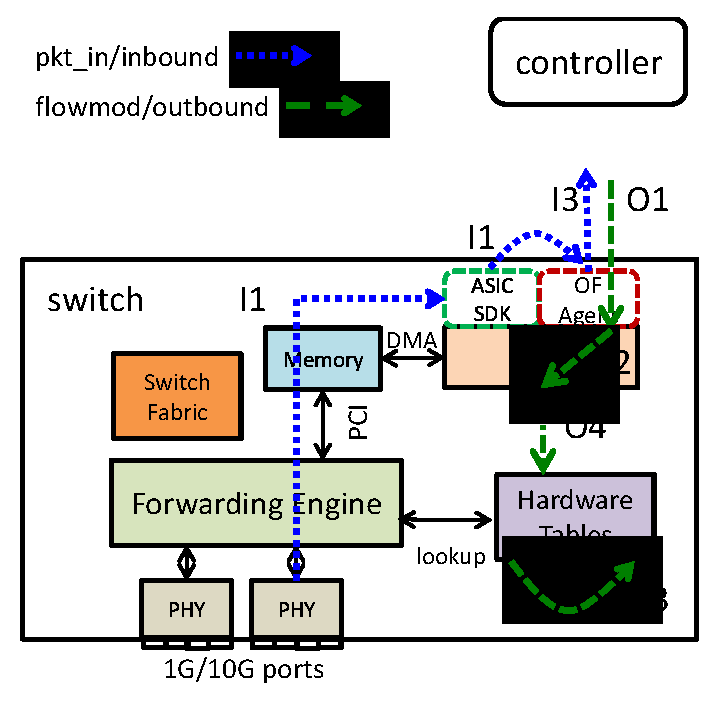
\epsfig{file=./figs/openflow_switch_illustrate.eps,width=0.4\textwidth}
% 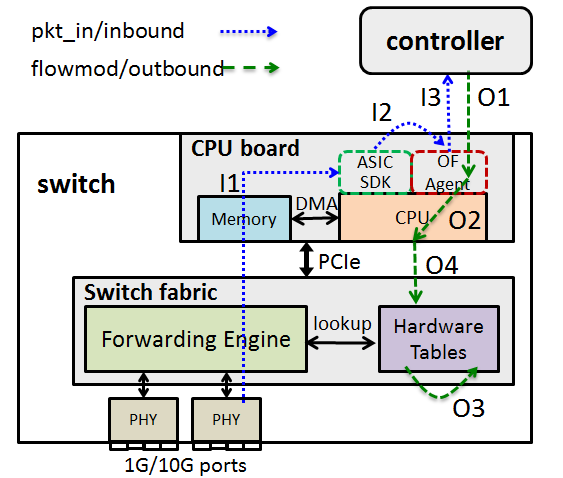
\includegraphics[width=3.5in]{figs/openflow_switch.PNG}
% \caption{Illustration of the t\_in and t\_out delay in an openflow switch.}\label{openflow_switch_delay}
% \end{figure}

% The first contribution of this paper is a systematic exploration of
% latencies in production SDN switches. We study switches from XXX
% \aditya{fill} different vendors under a variety of scenarios that
% carefully isolate the impact of different workload parameters on
% observed latencies. Further, we investigate the relationship between
% switch designs and observed latencies using both active greybox probes
% and feedback from hardware vendors. Key highlights from our
% measurements are as follows: (1) We find that t\_in delays can be as
% high as XXXXms.\aditya{fill} In some cases, poor software support for
% handling \packetin\ message may be an underlying cause, but we note
% that t\_in is always high whenever switch software is also processing
% \packetout\ and \flowmod\ messages. (2) We find that t\_out is
% unusually high as well: for example, inserting a burst of 50 rules
% into a switch based on the Broadcom chipset can take up to 100ms. TCAM
% hardware can support very fast updates, so this delay appears to arise
% primarily from switch software issues. \marina{such as when and what types of rules get puhsed into the TCAM} (3) Priorities can have a
% significant impact: inserting high priority rules into a table
% containing lower priority rules can take as long as XXXs.\aditya{fill}
% This is due to the memory chip's SDK rearranging rules in order of
% priority.

% Crucially, most of the root causes of the latencies are often not
% fundamental and arise due to poor switch software design. Only one
% root cause -- rule rearrangment in face of priorities -- appears to be
% linked to the hardware. A natural question to ask is whether switch
% vendors will improve their software such that most of the latencies we
% observe would go away. We don't believe this is likely: switch vendors
% will not put in the software design effort unless they see the outcome
% as a differentiator. Customers today continue to make purchase
% decisions mostly based on line speeds and perhaps flow table sizes,
% and hence it is likely that we're stuck at least in the near future
% with switch designs that are similar to what we have today.

% \fi
